\documentclass{beamer}
\usepackage{caption}
\usepackage{listings}
\usepackage[official]{eurosym}
% Remove the navigation buttons at the bottom right of each slide.
\setbeamertemplate{navigation symbols}{}
% Set bulletpoints to circles.
\setbeamertemplate{itemize items}[circle]

\title{Intro to Git}
\author{Netsoc}
% Remove the date.
\date{}
\begin{document}
\frame{\titlepage}

\section{Goals}
\begin{frame}
\frametitle{Goals}
\begin{itemize}
\item Introduce Git without assuming prior knowledge
\item Show you the 10\% of Git that can do 90\% of the work
\item Slides \& practical demonstration
\item Questions \& Answers (whenever you want)
\end{itemize}
\end{frame}

\section{Git}
\begin{frame}
\frametitle{Git}
\begin{itemize}
\item Version Control System (VCS)
\begin{itemize}
\item Keep track of changes in files over time
\item Track who changed what, when
\item Help multiple people work on the same files at the same time
\item Detect and sometimes resolve conflicts automatically
\end{itemize}
\item Created by Linus Torvalds in 2005 for Linux Kernel development
\item Command-line program, available on Linux, Mac and Windows https://git-scm.com/
\item Free and Open-Source
\item Once installed, just type "git" to get a list of useful commands
\end{itemize}
\end{frame}

\begin{frame}
\begin{figure}
\begin{center}
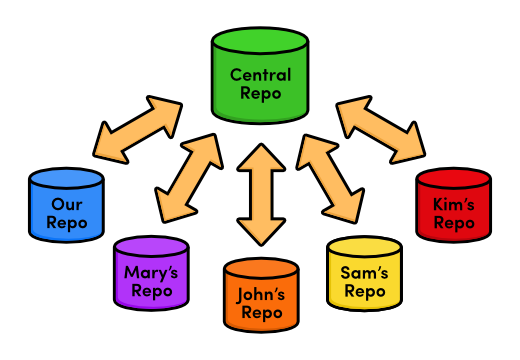
\includegraphics[scale=0.7]{centralised}
\caption{http://rypress.com/tutorials/git/media/8-7.png}
\end{center}
\end{figure}
\end{frame}

\begin{frame}
\frametitle{Github}
\begin{itemize}
\item A website for hosting git repositories
\item It's free
\item The user interface is great
\item Bug tracker, search function, can "star" and follow repositories
\end{itemize}
\end{frame}

\begin{frame}
\begin{figure}
\begin{center}
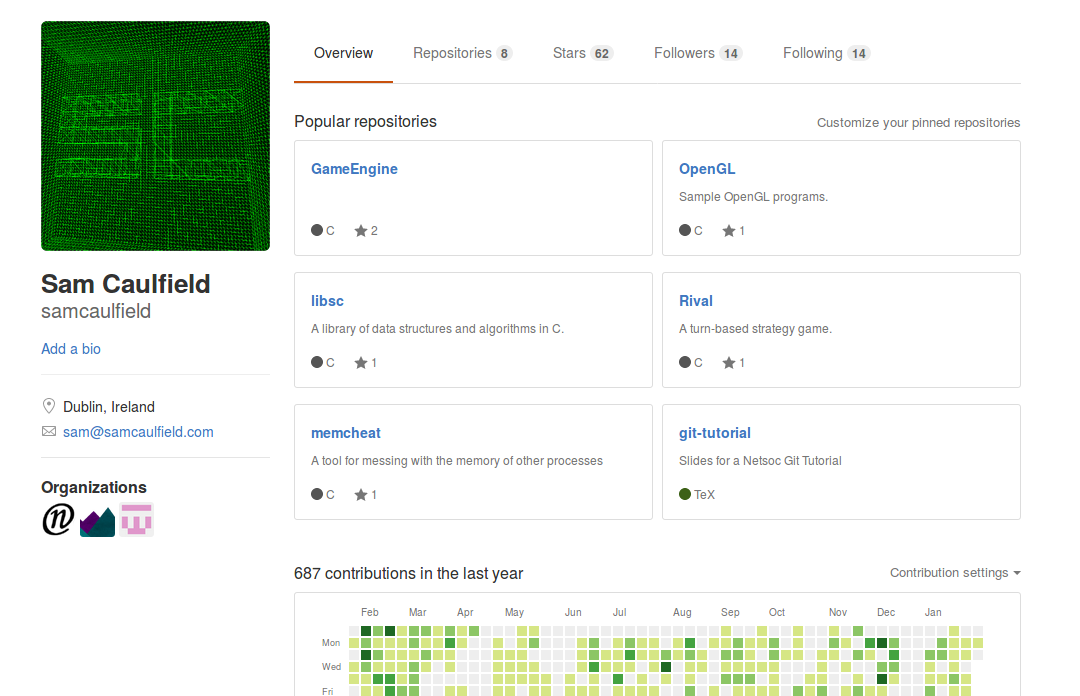
\includegraphics[scale=0.3]{githubmain}
\end{center}
\end{figure}
\end{frame}

\begin{frame}
\frametitle{How Git works}
\begin{itemize}
\item Git lives inside the .git folder in the project folder
\item This is where git keeps track of things for each project
\item Project developers don't need to touch this folder, it's for git only
\item Project developers only care about the human-readable files that we create
\end{itemize}
\end{frame}

\begin{frame}
\frametitle{Adding things to your repository}
\begin{itemize}
\item When you create or delete files, git doesn't automatically add or delete them from the repository
\item When you modify files, git doesn't automatically update the repository with the changes
\item You can make all the changes you want, and then turn to git when you're ready to commit them
\item This is good because it gives you time to think things through / clean up before uploading
\end{itemize}
\end{frame}

\section{Modifying your own repository}
\begin{frame}
\frametitle{Adding things to your repository}
\begin{itemize}
\item With Git, modifying your respository is manual
\item When you make changes, they only effect your copy of the repository
\item Changes are called "commits"
\item Then when you're ready, you upload the commits so your teammates can get them, and vice-versa
\end{itemize}
\end{frame}

\section{Getting a repository}
\begin{frame}
\frametitle{Getting a repository}
\begin{itemize}
\item Need to create or get a copy of the repository to begin working
\item to create: git init
\end{itemize}
\begin{figure}
\begin{center}
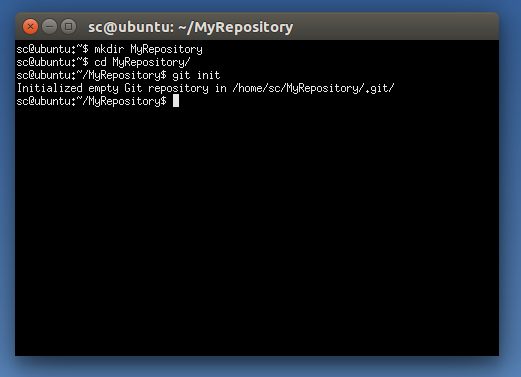
\includegraphics[scale=0.5]{gitinit}
\end{center}
\end{figure}
\end{frame}

\begin{frame}
\frametitle{Getting a repository}
\begin{itemize}
\item If you're not starting from scratch, need to get it from somewhere
\item to copy from somewhere else: git clone
\end{itemize}
\begin{figure}
\begin{center}
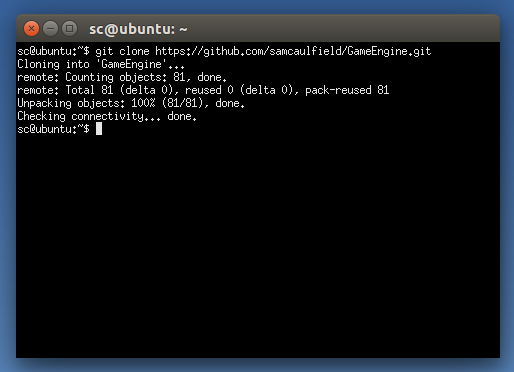
\includegraphics[scale=0.5]{gitclone}
\end{center}
\end{figure}
\end{frame}


\begin{frame}
\frametitle{Adding things to your repository}
\begin{itemize}
\item Git has the concept of a "staging area"
\item The purpose of the staging area is to gather up a set of changes to make a commit out of
\item By default changes to files are unstaged
\item You manually add files to the staging area
\item Then you can confirm the changes (commit)
\end{itemize}
\end{frame}

\begin{frame}
\begin{figure}
\begin{center}
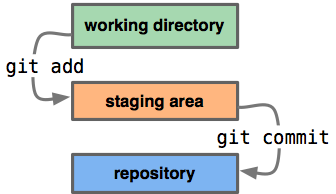
\includegraphics[scale=1.4]{stagingareadiagram}
\caption{http://codingdomain.com/git/partial-commits/git-staging-area.png}
\end{center}
\end{figure}
\end{frame}

\begin{frame}
\begin{figure}
\begin{center}
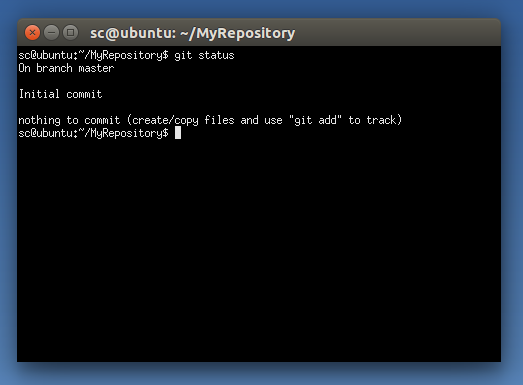
\includegraphics[scale=0.5]{gitstatus0}
\end{center}
\end{figure}
\end{frame}

\begin{frame}
\begin{figure}
\begin{center}
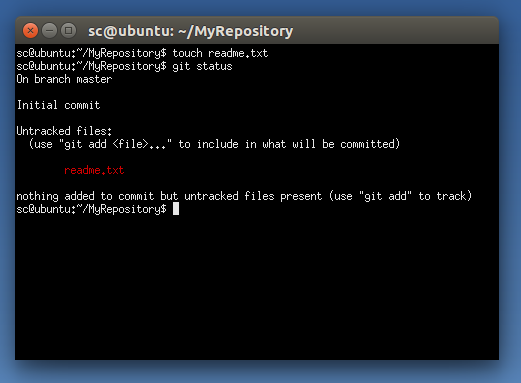
\includegraphics[scale=0.5]{gitstatus1}
\end{center}
\end{figure}
\end{frame}

\section{Staging files}
\begin{frame}
\begin{itemize}
\item Use the "git add" command (same as "git stage")
\item You can use "git add --patch" to add pieces of files
\end{itemize}
\begin{figure}
\begin{center}
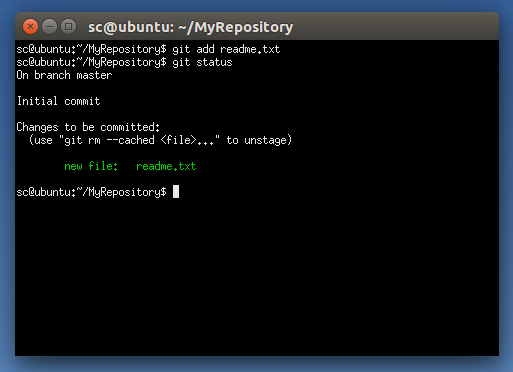
\includegraphics[scale=0.5]{gitadd0}
\end{center}
\end{figure}
\end{frame}

\begin{frame}
\frametitle{Staging files}
\begin{itemize}
\item You can add multiple files with wildcard (git add *)
\item This often goes wrong
\item .exe .bin .o .class .so etc.
\end{itemize}
\end{frame}

\begin{frame}
\frametitle{.gitignore}
\begin{itemize}
\item .gitignore file can mitigate this
\item .gitignore is a file you put in the repository
\item prevents people adding files that shouldn't go in the repository
\item one file type per line
\item git status won't show the files and they won't be used in wildcards
\end{itemize}
\end{frame}

\begin{frame}
\frametitle{Tracking files}
\begin{itemize}
\item Git tracks exactly what has changed in each file since the last "commit"
\item You can view unstaged changes with "git diff"
\item You can view staged changes with "git diff --staged"
\item You can view all changes with "git diff HEAD"
\end{itemize}
\end{frame}

\section{Unstaging changes}
\begin{frame}
\frametitle{Unstaging changes}
\begin{itemize}
\item You can unstage changes
\item Do this if you aren't ready to commit a change after all
\item This just takes the change out of the staging area, it doesn't delete it
\item Remember staging/unstaging != creating/deleting
\item The staging area is just showing Git your intent for the files
\item "git reset HEAD file"
\end{itemize}
\end{frame}

\section{Committing changes}
\begin{frame}
\frametitle{Committing changes}
\begin{itemize}
\item Staging/unstaging doesn't make permanent changes to the repository
\item That's what committing is for
\item Commits "lock in" staged changes
\item When you commit, the staged changes are converted to a commit
\item Git stores what each commit changed in it's .git folder
\item Before you make your first commit, you'll need to give Git some information
\end{itemize}
\end{frame}

\section{Git Config}
\begin{frame}
\frametitle{Git Config}
\begin{itemize}
\item Commits are summarised in a log
\item The log is a good record of the project's development history
\item All commits can be traced back to an author (name, date and email)
\item To tell Git how to "sign" your commits, use "git config"
\end{itemize}
\end{frame}

\section{Git Config}
\begin{frame}
\frametitle{Git Config}
\begin{figure}
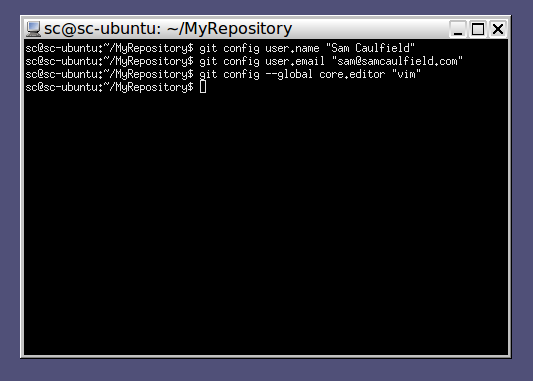
\includegraphics[scale=0.5]{gitconfig}
\end{figure}
\end{frame}

\section{Committing Changes}
\begin{frame}
\frametitle{Committing Changes}
\begin{itemize}
\item Now that the config is set up, you can commit
\item Use the "git commit" command
\item This gathers up the staged changes into a commit
\item You have to enter a commit message (for the log)
\end{itemize}
\begin{figure}
\end{figure}
\end{frame}

\section{Committing}
\begin{frame}
\frametitle{Committing}
\begin{figure}
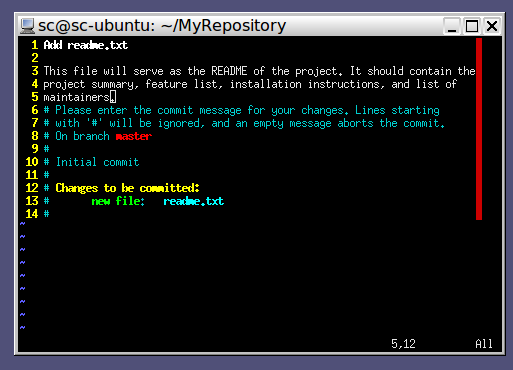
\includegraphics[scale=0.5]{committing}
\end{figure}
\end{frame}

\section{Git log}
\begin{frame}
\frametitle{Git Log}
\begin{itemize}
\item The "git log" tool is useful for showing a summary of commits
\item Remember the commits are the history
\item So a history of the commits is the history of the project
\end{itemize}
\begin{figure}
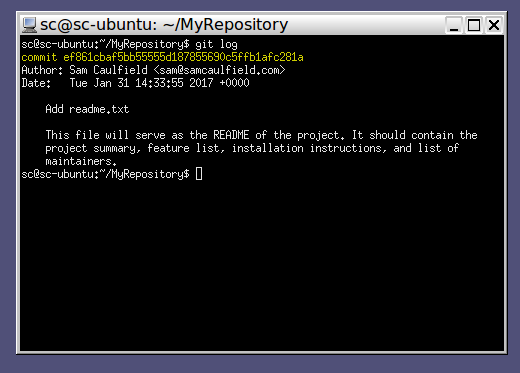
\includegraphics[scale=0.5]{gitlog0}
\end{figure}
\end{frame}

\section{Committing}
\begin{frame}
\frametitle{Committing Tips}
\begin{itemize}
\item Small and simple changes with good descriptions
\item Do one thing well
\item Should bring the repository from one consistent state to another
\item Be polished, i.e. code, tests and documentation where reasonable
\item Solving a problem often comes down to thinking what series of commits will it take to solve
\end{itemize}
\end{frame}

\begin{frame}
\frametitle{Commit Messages}
\begin{itemize}
\item The commits are the project history
\item So the commit messages are the more human-friendly project history
\item Explain why a change was made
\item Developer-to-developer communication
\end{itemize}
\end{frame}

\begin{frame}
\frametitle{Commit Messages}
\begin{itemize}
\item Title \& body
\item Personal preference \& project convention
\item The commit message "header" is generally kept to 50 chars or less
\item The header generally uses the imperative tense
\item "Add tests to maths library", "Fix bug in save dialog" etc.
\item The commit message body can be as long as you want
\item But is generally kept to 73 chars or less per line
\item http://chris.beams.io/posts/git-commit/
\end{itemize}
\begin{figure}
\end{figure}
\end{frame}

\section{Syncing your changes with other people}
\begin{frame}
\frametitle{Syncing your changes}
\begin{itemize}
\item Up to now we have only been modifying our own copy of the repository
\item To share the changes with your team you need to synchronise
\item This is done by downloading their changes "pulling"
\item and uploading your changes "pushing"
\item The "git pull" and "git push" commands do this
\end{itemize}
\end{frame}

\begin{frame}
\frametitle{Syncing your changes - remotes}
\begin{itemize}
\item To sync, you have to know where to pull/push changes from/to
\item In Git, servers that host repositories are called "remotes"
\item You can easily list the servers for your project with "git remote -v"
\item If you cloned a repository from Github, the remote is automatically set up for you
\end{itemize}
\begin{figure}
\end{figure}
\end{frame}

\begin{frame}
\frametitle{Git remotes}
\begin{figure}
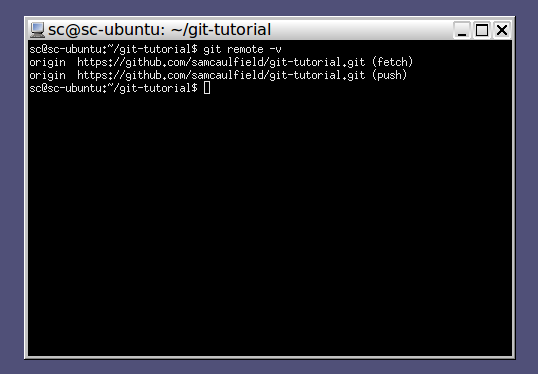
\includegraphics[scale=0.5]{gitremotev}
\end{figure}
\end{frame}

\begin{frame}
\frametitle{Pulling changes}
\begin{itemize}
\item You want to start the sync by pulling the new version of the repository
\item This is done with "git pull"
\item Generally speaking, you want to use "git pull --rebase"
\item git pull --rebase keeps the log history cleaner because it often doesn't produce a "merge commit"
\item Sometimes when you pull, conflicts can occur
\end{itemize}
\begin{figure}
\end{figure}
\end{frame}

\begin{frame}
\frametitle{Pushing changes}
\begin{itemize}
\item Once you've got up to date with the remote repository you'll want to push your changes
\item This is so your team members can access them
\item This is as simple as "git push"
\end{itemize}
\begin{figure}
\end{figure}
\end{frame}

\section{Workflow}
\begin{frame}
\frametitle{Merge Conflicts}
\begin{itemize}
\item Sometimes two people have modified the same part of the same file
\item This is a problem for the developers to solve, not Git
\item Git just highlights the conflict lines in the file and lets you solve it
\item This involves opening the file with the conflict in an editor and fixing it yourself
\item You then commit the fixed file
\item https://help.github.com/articles/resolving-a-merge-conflict-using-the-command-line/
\end{itemize}
\begin{figure}
\end{figure}
\end{frame}

\begin{frame}
\frametitle{Merge Conflicts}
\begin{itemize}
\item Merge conflicts can often be avoided by better project management
\item Two people shouldn't really be modifying the same bits of the same file too often
\item Can have the concept of "file owners"
\item One person or team responsible for changing particular files
\end{itemize}
\end{frame}

\begin{frame}
\frametitle{Branches}
\begin{itemize}
\item A branch is like a private copy of the repository
\item Each person can have multiple branches, and can share the branches with others
\item Every project has at least one branch, just one is fine though
\item One branch is usually considered the One True Branch (called "master")
\item The master branch usually has the latest stable version of the project
\end{itemize}
\begin{figure}
\end{figure}
\end{frame}

\begin{frame}
\frametitle{Branches}
\begin{itemize}
\item Not really worth worrying about just starting out
\item Can be quite useful for large projects
\item Can create a branch to do a feature, and it hides the messy commits away
\item General use case is: create branch, implement feature, merge branch into master and delete branch
\end{itemize}
\end{frame}

\begin{frame}
\frametitle{Branches}
\begin{itemize}
\item "git branch branchname" - create a branch
\item "git branch -d branchname" - delete a branch
\item "git checkout branchname" - switch to that branch
\item Before we were doing everything on the master branch
\item Same commands apply to all branches
\end{itemize}
\begin{figure}
\end{figure}
\end{frame}

\begin{frame}
\frametitle{Forks}
\begin{itemize}
\item Different to branches
\item Not a concept that the git program deals with
\item A fork is a term for when a whole project is copied and worked on by someone else
\item e.g. Ubuntu started as a fork of Debian
\item It's more of a people term than a technical term
\end{itemize}
\begin{figure}
\end{figure}
\end{frame}

\begin{frame}
\frametitle{Pull request}
\begin{itemize}
\item A git term where someone makes a contribution to a project that they don't have push access on
\item A project maintainer has to manually approve the change and pull it
\item A good way to accept contributions from the public
\item Github has a nice user interface for this
\end{itemize}
\begin{figure}
\end{figure}
\end{frame}

\begin{frame}
\frametitle{Tags}
\begin{itemize}
\item In git you can "tag" certain commits
\item This can be to tag release versions
\item You can tag the current commit with `git tag -a v1.0 -m "beta release"`
\item This can make it easier to keep track of stable versions of the project
\end{itemize}
\begin{figure}
\end{figure}
\end{frame}

\end{document}

